% Options for packages loaded elsewhere
\PassOptionsToPackage{unicode}{hyperref}
\PassOptionsToPackage{hyphens}{url}
\PassOptionsToPackage{dvipsnames,svgnames,x11names}{xcolor}
%
\documentclass[
  letterpaper,
  DIV=11,
  numbers=noendperiod]{scrartcl}

\usepackage{amsmath,amssymb}
\usepackage{iftex}
\ifPDFTeX
  \usepackage[T1]{fontenc}
  \usepackage[utf8]{inputenc}
  \usepackage{textcomp} % provide euro and other symbols
\else % if luatex or xetex
  \usepackage{unicode-math}
  \defaultfontfeatures{Scale=MatchLowercase}
  \defaultfontfeatures[\rmfamily]{Ligatures=TeX,Scale=1}
\fi
\usepackage{lmodern}
\ifPDFTeX\else  
    % xetex/luatex font selection
\fi
% Use upquote if available, for straight quotes in verbatim environments
\IfFileExists{upquote.sty}{\usepackage{upquote}}{}
\IfFileExists{microtype.sty}{% use microtype if available
  \usepackage[]{microtype}
  \UseMicrotypeSet[protrusion]{basicmath} % disable protrusion for tt fonts
}{}
\makeatletter
\@ifundefined{KOMAClassName}{% if non-KOMA class
  \IfFileExists{parskip.sty}{%
    \usepackage{parskip}
  }{% else
    \setlength{\parindent}{0pt}
    \setlength{\parskip}{6pt plus 2pt minus 1pt}}
}{% if KOMA class
  \KOMAoptions{parskip=half}}
\makeatother
\usepackage{xcolor}
\setlength{\emergencystretch}{3em} % prevent overfull lines
\setcounter{secnumdepth}{-\maxdimen} % remove section numbering
% Make \paragraph and \subparagraph free-standing
\makeatletter
\ifx\paragraph\undefined\else
  \let\oldparagraph\paragraph
  \renewcommand{\paragraph}{
    \@ifstar
      \xxxParagraphStar
      \xxxParagraphNoStar
  }
  \newcommand{\xxxParagraphStar}[1]{\oldparagraph*{#1}\mbox{}}
  \newcommand{\xxxParagraphNoStar}[1]{\oldparagraph{#1}\mbox{}}
\fi
\ifx\subparagraph\undefined\else
  \let\oldsubparagraph\subparagraph
  \renewcommand{\subparagraph}{
    \@ifstar
      \xxxSubParagraphStar
      \xxxSubParagraphNoStar
  }
  \newcommand{\xxxSubParagraphStar}[1]{\oldsubparagraph*{#1}\mbox{}}
  \newcommand{\xxxSubParagraphNoStar}[1]{\oldsubparagraph{#1}\mbox{}}
\fi
\makeatother

\usepackage{color}
\usepackage{fancyvrb}
\newcommand{\VerbBar}{|}
\newcommand{\VERB}{\Verb[commandchars=\\\{\}]}
\DefineVerbatimEnvironment{Highlighting}{Verbatim}{commandchars=\\\{\}}
% Add ',fontsize=\small' for more characters per line
\usepackage{framed}
\definecolor{shadecolor}{RGB}{241,243,245}
\newenvironment{Shaded}{\begin{snugshade}}{\end{snugshade}}
\newcommand{\AlertTok}[1]{\textcolor[rgb]{0.68,0.00,0.00}{#1}}
\newcommand{\AnnotationTok}[1]{\textcolor[rgb]{0.37,0.37,0.37}{#1}}
\newcommand{\AttributeTok}[1]{\textcolor[rgb]{0.40,0.45,0.13}{#1}}
\newcommand{\BaseNTok}[1]{\textcolor[rgb]{0.68,0.00,0.00}{#1}}
\newcommand{\BuiltInTok}[1]{\textcolor[rgb]{0.00,0.23,0.31}{#1}}
\newcommand{\CharTok}[1]{\textcolor[rgb]{0.13,0.47,0.30}{#1}}
\newcommand{\CommentTok}[1]{\textcolor[rgb]{0.37,0.37,0.37}{#1}}
\newcommand{\CommentVarTok}[1]{\textcolor[rgb]{0.37,0.37,0.37}{\textit{#1}}}
\newcommand{\ConstantTok}[1]{\textcolor[rgb]{0.56,0.35,0.01}{#1}}
\newcommand{\ControlFlowTok}[1]{\textcolor[rgb]{0.00,0.23,0.31}{\textbf{#1}}}
\newcommand{\DataTypeTok}[1]{\textcolor[rgb]{0.68,0.00,0.00}{#1}}
\newcommand{\DecValTok}[1]{\textcolor[rgb]{0.68,0.00,0.00}{#1}}
\newcommand{\DocumentationTok}[1]{\textcolor[rgb]{0.37,0.37,0.37}{\textit{#1}}}
\newcommand{\ErrorTok}[1]{\textcolor[rgb]{0.68,0.00,0.00}{#1}}
\newcommand{\ExtensionTok}[1]{\textcolor[rgb]{0.00,0.23,0.31}{#1}}
\newcommand{\FloatTok}[1]{\textcolor[rgb]{0.68,0.00,0.00}{#1}}
\newcommand{\FunctionTok}[1]{\textcolor[rgb]{0.28,0.35,0.67}{#1}}
\newcommand{\ImportTok}[1]{\textcolor[rgb]{0.00,0.46,0.62}{#1}}
\newcommand{\InformationTok}[1]{\textcolor[rgb]{0.37,0.37,0.37}{#1}}
\newcommand{\KeywordTok}[1]{\textcolor[rgb]{0.00,0.23,0.31}{\textbf{#1}}}
\newcommand{\NormalTok}[1]{\textcolor[rgb]{0.00,0.23,0.31}{#1}}
\newcommand{\OperatorTok}[1]{\textcolor[rgb]{0.37,0.37,0.37}{#1}}
\newcommand{\OtherTok}[1]{\textcolor[rgb]{0.00,0.23,0.31}{#1}}
\newcommand{\PreprocessorTok}[1]{\textcolor[rgb]{0.68,0.00,0.00}{#1}}
\newcommand{\RegionMarkerTok}[1]{\textcolor[rgb]{0.00,0.23,0.31}{#1}}
\newcommand{\SpecialCharTok}[1]{\textcolor[rgb]{0.37,0.37,0.37}{#1}}
\newcommand{\SpecialStringTok}[1]{\textcolor[rgb]{0.13,0.47,0.30}{#1}}
\newcommand{\StringTok}[1]{\textcolor[rgb]{0.13,0.47,0.30}{#1}}
\newcommand{\VariableTok}[1]{\textcolor[rgb]{0.07,0.07,0.07}{#1}}
\newcommand{\VerbatimStringTok}[1]{\textcolor[rgb]{0.13,0.47,0.30}{#1}}
\newcommand{\WarningTok}[1]{\textcolor[rgb]{0.37,0.37,0.37}{\textit{#1}}}

\providecommand{\tightlist}{%
  \setlength{\itemsep}{0pt}\setlength{\parskip}{0pt}}\usepackage{longtable,booktabs,array}
\usepackage{calc} % for calculating minipage widths
% Correct order of tables after \paragraph or \subparagraph
\usepackage{etoolbox}
\makeatletter
\patchcmd\longtable{\par}{\if@noskipsec\mbox{}\fi\par}{}{}
\makeatother
% Allow footnotes in longtable head/foot
\IfFileExists{footnotehyper.sty}{\usepackage{footnotehyper}}{\usepackage{footnote}}
\makesavenoteenv{longtable}
\usepackage{graphicx}
\makeatletter
\newsavebox\pandoc@box
\newcommand*\pandocbounded[1]{% scales image to fit in text height/width
  \sbox\pandoc@box{#1}%
  \Gscale@div\@tempa{\textheight}{\dimexpr\ht\pandoc@box+\dp\pandoc@box\relax}%
  \Gscale@div\@tempb{\linewidth}{\wd\pandoc@box}%
  \ifdim\@tempb\p@<\@tempa\p@\let\@tempa\@tempb\fi% select the smaller of both
  \ifdim\@tempa\p@<\p@\scalebox{\@tempa}{\usebox\pandoc@box}%
  \else\usebox{\pandoc@box}%
  \fi%
}
% Set default figure placement to htbp
\def\fps@figure{htbp}
\makeatother

\usepackage{float}
\usepackage{tabularray}
\usepackage[normalem]{ulem}
\usepackage{graphicx}
\UseTblrLibrary{booktabs}
\UseTblrLibrary{rotating}
\UseTblrLibrary{siunitx}
\NewTableCommand{\tinytableDefineColor}[3]{\definecolor{#1}{#2}{#3}}
\newcommand{\tinytableTabularrayUnderline}[1]{\underline{#1}}
\newcommand{\tinytableTabularrayStrikeout}[1]{\sout{#1}}
\usepackage{fvextra}
\DefineVerbatimEnvironment{Highlighting}{Verbatim}{breaklines,commandchars=\\\{\}}
\DefineVerbatimEnvironment{OutputCode}{Verbatim}{breaklines,commandchars=\\\{\}}
\KOMAoption{captions}{tableheading}
\makeatletter
\@ifpackageloaded{caption}{}{\usepackage{caption}}
\AtBeginDocument{%
\ifdefined\contentsname
  \renewcommand*\contentsname{Table of contents}
\else
  \newcommand\contentsname{Table of contents}
\fi
\ifdefined\listfigurename
  \renewcommand*\listfigurename{List of Figures}
\else
  \newcommand\listfigurename{List of Figures}
\fi
\ifdefined\listtablename
  \renewcommand*\listtablename{List of Tables}
\else
  \newcommand\listtablename{List of Tables}
\fi
\ifdefined\figurename
  \renewcommand*\figurename{Figure}
\else
  \newcommand\figurename{Figure}
\fi
\ifdefined\tablename
  \renewcommand*\tablename{Table}
\else
  \newcommand\tablename{Table}
\fi
}
\@ifpackageloaded{float}{}{\usepackage{float}}
\floatstyle{ruled}
\@ifundefined{c@chapter}{\newfloat{codelisting}{h}{lop}}{\newfloat{codelisting}{h}{lop}[chapter]}
\floatname{codelisting}{Listing}
\newcommand*\listoflistings{\listof{codelisting}{List of Listings}}
\makeatother
\makeatletter
\makeatother
\makeatletter
\@ifpackageloaded{caption}{}{\usepackage{caption}}
\@ifpackageloaded{subcaption}{}{\usepackage{subcaption}}
\makeatother

\usepackage{bookmark}

\IfFileExists{xurl.sty}{\usepackage{xurl}}{} % add URL line breaks if available
\urlstyle{same} % disable monospaced font for URLs
\hypersetup{
  pdftitle={Problem set 4},
  pdfauthor={Hyoungchul Kim},
  colorlinks=true,
  linkcolor={blue},
  filecolor={Maroon},
  citecolor={Blue},
  urlcolor={Blue},
  pdfcreator={LaTeX via pandoc}}


\title{Problem set 4}
\author{Hyoungchul Kim}
\date{2025-04-12}

\begin{document}
\maketitle


Read in the data

\begin{Shaded}
\begin{Highlighting}[]
\FunctionTok{library}\NormalTok{(tidyverse)}
\FunctionTok{library}\NormalTok{(data.table)}
\FunctionTok{library}\NormalTok{(fixest)}
\FunctionTok{library}\NormalTok{(texreg) }

\NormalTok{data4 }\OtherTok{\textless{}{-}}\NormalTok{ haven}\SpecialCharTok{::}\FunctionTok{read\_dta}\NormalTok{(}\StringTok{"data/final4.dta"}\NormalTok{, }\AttributeTok{encoding =} \StringTok{"latin1"}\NormalTok{)}
\NormalTok{data5 }\OtherTok{\textless{}{-}}\NormalTok{ haven}\SpecialCharTok{::}\FunctionTok{read\_dta}\NormalTok{(}\StringTok{"data/final5.dta"}\NormalTok{, }\AttributeTok{encoding =} \StringTok{"latin1"}\NormalTok{)}

\NormalTok{data4 }\OtherTok{\textless{}{-}}\NormalTok{ data4 }\SpecialCharTok{\%\textgreater{}\%} \FunctionTok{mutate}\NormalTok{(}
  \AttributeTok{avgverb =} \FunctionTok{ifelse}\NormalTok{(avgverb }\SpecialCharTok{\textgreater{}} \DecValTok{100}\NormalTok{, avgverb }\SpecialCharTok{{-}} \DecValTok{100}\NormalTok{, avgverb),}
  \AttributeTok{avgmath =} \FunctionTok{ifelse}\NormalTok{(avgmath }\SpecialCharTok{\textgreater{}} \DecValTok{100}\NormalTok{, avgmath }\SpecialCharTok{{-}} \DecValTok{100}\NormalTok{, avgmath)) }\SpecialCharTok{\%\textgreater{}\%} 
  \FunctionTok{filter}\NormalTok{(classize }\SpecialCharTok{\textgreater{}} \DecValTok{1} \SpecialCharTok{\&}\NormalTok{ classize }\SpecialCharTok{\textless{}} \DecValTok{45} \SpecialCharTok{\&}\NormalTok{ c\_size }\SpecialCharTok{\textgreater{}} \DecValTok{5}\NormalTok{) }\SpecialCharTok{\%\textgreater{}\%} 
  \FunctionTok{filter}\NormalTok{(c\_leom }\SpecialCharTok{==} \DecValTok{1} \SpecialCharTok{\&}\NormalTok{ c\_pik }\SpecialCharTok{\textless{}} \DecValTok{3}\NormalTok{)}

\NormalTok{data5 }\OtherTok{\textless{}{-}}\NormalTok{ data5 }\SpecialCharTok{\%\textgreater{}\%} \FunctionTok{mutate}\NormalTok{(}
  \AttributeTok{avgverb =} \FunctionTok{ifelse}\NormalTok{(avgverb }\SpecialCharTok{\textgreater{}} \DecValTok{100}\NormalTok{, avgverb }\SpecialCharTok{{-}} \DecValTok{100}\NormalTok{, avgverb),}
  \AttributeTok{avgmath =} \FunctionTok{ifelse}\NormalTok{(avgmath }\SpecialCharTok{\textgreater{}} \DecValTok{100}\NormalTok{, avgmath }\SpecialCharTok{{-}} \DecValTok{100}\NormalTok{, avgmath)) }\SpecialCharTok{\%\textgreater{}\%} 
  \FunctionTok{filter}\NormalTok{(classize }\SpecialCharTok{\textgreater{}} \DecValTok{1} \SpecialCharTok{\&}\NormalTok{ classize }\SpecialCharTok{\textless{}}\DecValTok{45} \SpecialCharTok{\&}\NormalTok{ c\_size }\SpecialCharTok{\textgreater{}} \DecValTok{5}\NormalTok{) }\SpecialCharTok{\%\textgreater{}\%} 
  \FunctionTok{filter}\NormalTok{(c\_leom }\SpecialCharTok{==} \DecValTok{1} \SpecialCharTok{\&}\NormalTok{ c\_pik }\SpecialCharTok{\textless{}} \DecValTok{3}\NormalTok{)}
\end{Highlighting}
\end{Shaded}

\subsection{Q1}\label{q1}

I have read the QJE article.

\subsection{Q2}\label{q2}

We do simple regression as follows:

\begin{Shaded}
\begin{Highlighting}[]
\NormalTok{models }\OtherTok{\textless{}{-}} \FunctionTok{list}\NormalTok{(}
  \FunctionTok{feols}\NormalTok{(avgverb }\SpecialCharTok{\textasciitilde{}}\NormalTok{ classize, }\AttributeTok{data =}\NormalTok{ data4, }\AttributeTok{cluster =} \SpecialCharTok{\textasciitilde{}}\NormalTok{schlcode),}
  \FunctionTok{feols}\NormalTok{(avgmath }\SpecialCharTok{\textasciitilde{}}\NormalTok{ classize, }\AttributeTok{data =}\NormalTok{ data4, }\AttributeTok{cluster =} \SpecialCharTok{\textasciitilde{}}\NormalTok{schlcode),}
  \FunctionTok{feols}\NormalTok{(avgverb }\SpecialCharTok{\textasciitilde{}}\NormalTok{ classize, }\AttributeTok{data =}\NormalTok{ data5, }\AttributeTok{cluster =} \SpecialCharTok{\textasciitilde{}}\NormalTok{schlcode),}
  \FunctionTok{feols}\NormalTok{(avgmath }\SpecialCharTok{\textasciitilde{}}\NormalTok{ classize, }\AttributeTok{data =}\NormalTok{ data5, }\AttributeTok{cluster =} \SpecialCharTok{\textasciitilde{}}\NormalTok{schlcode))  }

\FunctionTok{library}\NormalTok{(modelsummary)}

\CommentTok{\# modelsummary(models,}
\CommentTok{\#   starts = TRUE,}
\CommentTok{\#   statistic = "(\{std.error\})",}
\CommentTok{\#   gof\_omit = "R2|Adj|Log|AIC|BIC|RMSE",}
\CommentTok{\#   output = "latex",}
\CommentTok{\#   coef\_rename = c("c\_size" = "Class Size", "(Intercept)" = "Constant"),}
\CommentTok{\#   title = "Bivariate Regressions of Test Scores on Class Size",}
\CommentTok{\#   notes = "*p \textless{} 0.05, ** p \textless{} 0.01, *** p \textless{} 0.001",}
\CommentTok{\#   add\_rows = tibble(}
\CommentTok{\#     Term = "Observations",}
\CommentTok{\#     \textasciigrave{}Model 1\textasciigrave{} = nobs(models[[1]]),}
\CommentTok{\#     \textasciigrave{}Model 2\textasciigrave{} = nobs(models[[2]]),}
\CommentTok{\#     \textasciigrave{}Model 3\textasciigrave{} = nobs(models[[3]]),}
\CommentTok{\#     \textasciigrave{}Model 4\textasciigrave{} = nobs(models[[4]])}
\CommentTok{\#   ), output = "latex")}

\FunctionTok{screenreg}\NormalTok{(models, }
  \AttributeTok{custom.model.names =} \FunctionTok{c}\NormalTok{(}\StringTok{"Grammar {-} 4th"}\NormalTok{, }\StringTok{"Math {-} 4th"}\NormalTok{, }\StringTok{"Grammar {-} 5th"}\NormalTok{, }\StringTok{"Math {-} 5th"}\NormalTok{),}
  \AttributeTok{custom.coef.map =} \FunctionTok{list}\NormalTok{(}\StringTok{"classize"} \OtherTok{=} \StringTok{"Class size"}\NormalTok{),}
  \AttributeTok{include.adjrs =} \ConstantTok{FALSE}\NormalTok{, }\AttributeTok{include.proj.stats =} \ConstantTok{FALSE}\NormalTok{, }\AttributeTok{include.groups =} \ConstantTok{FALSE}\NormalTok{)}
\end{Highlighting}
\end{Shaded}

\begin{verbatim}

==================================================================
            Grammar - 4th  Math - 4th   Grammar - 5th  Math - 5th 
------------------------------------------------------------------
Class size     0.14 ***       0.22 ***     0.22 ***       0.33 ***
              (0.03)         (0.04)       (0.03)         (0.04)   
------------------------------------------------------------------
Num. obs.   2049           2049         2019           2019       
R^2            0.01           0.03         0.04           0.05    
==================================================================
*** p < 0.001; ** p < 0.01; * p < 0.05
\end{verbatim}

The results show that larger class sizes are associated with higher test
scores. This is quite counterintuitive and it is probably because of
some endogeneity issue. One possible issue might be that schools are
assigning underperforming students in small classes to boost their
performance. In this case, the result could be biased as underperforming
students will tend to get better but will still be performing less than
other students.

\subsection{Q3}\label{q3}

We plot the predictions of Maimonides' rule:

\begin{Shaded}
\begin{Highlighting}[]
\NormalTok{data4 }\OtherTok{\textless{}{-}}\NormalTok{ data4 }\SpecialCharTok{\%\textgreater{}\%} \FunctionTok{mutate}\NormalTok{(}\AttributeTok{grade =} \DecValTok{4}\NormalTok{)}
\NormalTok{data5 }\OtherTok{\textless{}{-}}\NormalTok{ data5 }\SpecialCharTok{\%\textgreater{}\%} \FunctionTok{mutate}\NormalTok{(}\AttributeTok{grade =} \DecValTok{5}\NormalTok{)}

\NormalTok{data }\OtherTok{\textless{}{-}}\NormalTok{ data4 }\SpecialCharTok{\%\textgreater{}\%} \FunctionTok{bind\_rows}\NormalTok{(data5)}

\NormalTok{label\_map }\OtherTok{\textless{}{-}} \FunctionTok{c}\NormalTok{(}\StringTok{"4"} \OtherTok{=} \StringTok{"4th grade"}\NormalTok{, }\StringTok{"5"} \OtherTok{=} \StringTok{"5th grade"}\NormalTok{)}

\NormalTok{data }\SpecialCharTok{\%\textgreater{}\%}  
  \FunctionTok{ggplot}\NormalTok{(}\FunctionTok{aes}\NormalTok{(}\AttributeTok{x =}\NormalTok{ c\_size, }\AttributeTok{y =} \FunctionTok{trunc}\NormalTok{((c\_size }\SpecialCharTok{{-}} \DecValTok{1}\NormalTok{) }\SpecialCharTok{/} \DecValTok{40}\NormalTok{) }\SpecialCharTok{+} \DecValTok{1}\NormalTok{)) }\SpecialCharTok{+}
  \FunctionTok{geom\_point}\NormalTok{() }\SpecialCharTok{+}
  \FunctionTok{scale\_x\_continuous}\NormalTok{(}\AttributeTok{name =} \StringTok{"School{-}grade enrollment"}\NormalTok{, }\AttributeTok{breaks =} \FunctionTok{c}\NormalTok{(}\DecValTok{0}\NormalTok{, }\DecValTok{40}\NormalTok{, }\DecValTok{50}\NormalTok{, }\DecValTok{80}\NormalTok{, }\DecValTok{100}\NormalTok{, }\DecValTok{120}\NormalTok{, }\DecValTok{150}\NormalTok{, }\DecValTok{160}\NormalTok{, }\DecValTok{200}\NormalTok{, }\DecValTok{200}\NormalTok{, }\DecValTok{250}\NormalTok{)) }\SpecialCharTok{+}
  \FunctionTok{scale\_y\_continuous}\NormalTok{(}\AttributeTok{name =} \StringTok{"Predicted number of classes"}\NormalTok{, }\AttributeTok{breaks=}\DecValTok{1}\SpecialCharTok{:}\DecValTok{6}\NormalTok{) }\SpecialCharTok{+}
  \FunctionTok{facet\_wrap}\NormalTok{(}\SpecialCharTok{\textasciitilde{}}\NormalTok{grade, }\AttributeTok{nrow =} \DecValTok{2}\NormalTok{, }\AttributeTok{labeller =} \FunctionTok{labeller}\NormalTok{(}\AttributeTok{grade =}\NormalTok{ label\_map)) }\SpecialCharTok{+}
  \FunctionTok{theme\_bw}\NormalTok{()}
\end{Highlighting}
\end{Shaded}

\pandocbounded{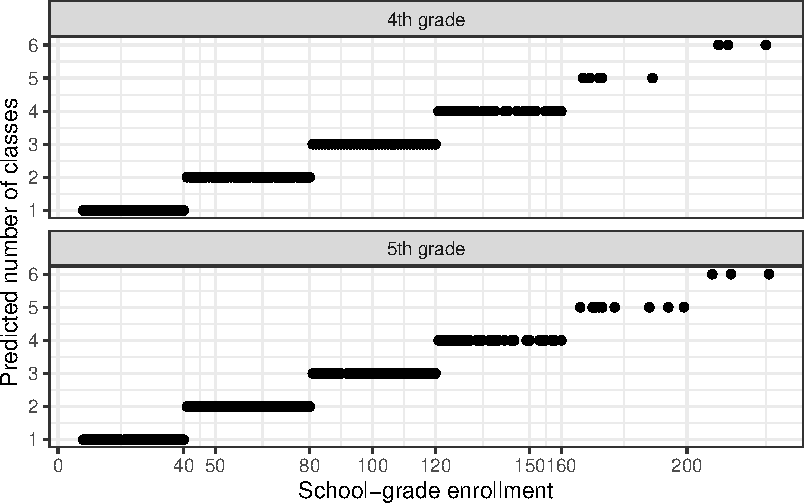
\includegraphics[keepaspectratio]{report_files/figure-pdf/unnamed-chunk-3-1.pdf}}

\begin{Shaded}
\begin{Highlighting}[]
\NormalTok{data }\SpecialCharTok{\%\textgreater{}\%}  
  \FunctionTok{ggplot}\NormalTok{(}\FunctionTok{aes}\NormalTok{(}\AttributeTok{x =}\NormalTok{ c\_size, }\AttributeTok{y =}\NormalTok{ c\_size }\SpecialCharTok{/}\NormalTok{ (}\FunctionTok{trunc}\NormalTok{((c\_size }\SpecialCharTok{{-}} \DecValTok{1}\NormalTok{) }\SpecialCharTok{/} \DecValTok{40}\NormalTok{) }\SpecialCharTok{+} \DecValTok{1}\NormalTok{))) }\SpecialCharTok{+}
  \FunctionTok{geom\_point}\NormalTok{() }\SpecialCharTok{+}
  \FunctionTok{scale\_x\_continuous}\NormalTok{(}\AttributeTok{name =} \StringTok{"School{-}grade enrollment"}\NormalTok{, }\AttributeTok{breaks =} \FunctionTok{c}\NormalTok{(}\DecValTok{0}\NormalTok{, }\DecValTok{40}\NormalTok{, }\DecValTok{50}\NormalTok{, }\DecValTok{80}\NormalTok{, }\DecValTok{100}\NormalTok{, }\DecValTok{120}\NormalTok{, }\DecValTok{150}\NormalTok{, }\DecValTok{160}\NormalTok{, }\DecValTok{200}\NormalTok{, }\DecValTok{200}\NormalTok{, }\DecValTok{250}\NormalTok{)) }\SpecialCharTok{+}
  \FunctionTok{scale\_y\_continuous}\NormalTok{(}\AttributeTok{name =} \StringTok{"Predicted number of classes"}\NormalTok{, }\AttributeTok{breaks=}\FunctionTok{seq}\NormalTok{(}\AttributeTok{from=}\DecValTok{10}\NormalTok{, }\AttributeTok{to =} \DecValTok{45}\NormalTok{, }\AttributeTok{by =} \DecValTok{10}\NormalTok{)) }\SpecialCharTok{+}
  \FunctionTok{facet\_wrap}\NormalTok{(}\SpecialCharTok{\textasciitilde{}}\NormalTok{grade, }\AttributeTok{nrow =} \DecValTok{2}\NormalTok{, }\AttributeTok{labeller =} \FunctionTok{labeller}\NormalTok{(}\AttributeTok{grade =}\NormalTok{ label\_map)) }\SpecialCharTok{+}
  \FunctionTok{theme\_bw}\NormalTok{()}
\end{Highlighting}
\end{Shaded}

\pandocbounded{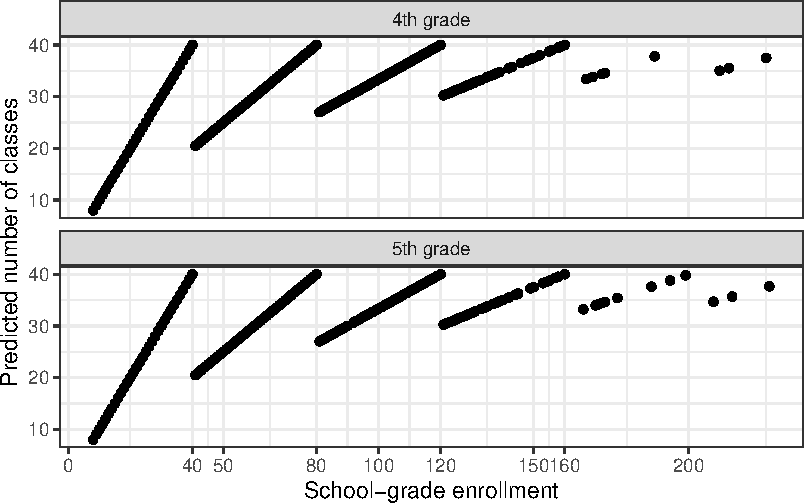
\includegraphics[keepaspectratio]{report_files/figure-pdf/unnamed-chunk-4-1.pdf}}

From the figures, we can see that potential sources of variation in
class size that might be useful are the discrete jumps happening around
enrollment in multiples of 40. If we compare classses close to the
either side of the cutoff, we could assume that these classes are
similar to each other along all other dimensions except for the class
size induced by the cutoff rule. Thus we could use the class size rule
as the exogenous variation to study the impact of class size on other
outcomes.

\clearpage

\subsection{Q4}\label{q4}

Descriptive statistics on mean class size students actually face is as
follows:

\clearpage

\begin{Shaded}
\begin{Highlighting}[]
\NormalTok{data\_m }\OtherTok{\textless{}{-}}\NormalTok{ data }\SpecialCharTok{\%\textgreater{}\%} 
  \FunctionTok{group\_by}\NormalTok{(c\_size) }\SpecialCharTok{\%\textgreater{}\%} 
  \FunctionTok{summarise}\NormalTok{(}\AttributeTok{mean\_class =} \FunctionTok{mean}\NormalTok{(classize, }\AttributeTok{na.rm=}\NormalTok{T), }\AttributeTok{.groups =} \StringTok{"drop"}\NormalTok{) }\SpecialCharTok{\%\textgreater{}\%} 
  \FunctionTok{rename}\NormalTok{(}\StringTok{"Mean class size"} \OtherTok{=} \StringTok{"mean\_class"}\NormalTok{)}

\FunctionTok{datasummary}\NormalTok{(}\StringTok{\textasciigrave{}}\AttributeTok{Mean class size}\StringTok{\textasciigrave{}} \SpecialCharTok{\textasciitilde{}}\NormalTok{ mean }\SpecialCharTok{+}\NormalTok{ sd }\SpecialCharTok{+}\NormalTok{ median }\SpecialCharTok{+}\NormalTok{ min }\SpecialCharTok{+}\NormalTok{ max, }\AttributeTok{data =}\NormalTok{ data\_m)}
\end{Highlighting}
\end{Shaded}

\begin{table}
\centering
\begin{tblr}[         %% tabularray outer open
]                     %% tabularray outer close
{                     %% tabularray inner open
colspec={Q[]Q[]Q[]Q[]Q[]Q[]},
column{1}={}{halign=l,},
column{2,3,4,5,6}={}{halign=r,},
}                     %% tabularray inner close
\toprule
& mean & sd & median & min & max \\ \midrule %% TinyTableHeader
Mean class size & \num{30.63} & \num{6.38} & \num{32.34} & \num{8.00} & \num{39.92} \\
\bottomrule
\end{tblr}
\end{table}

I also graph the actual and predicted average class size by enrollment
as follows:

\begin{Shaded}
\begin{Highlighting}[]
\NormalTok{data\_m }\OtherTok{\textless{}{-}}\NormalTok{ data }\SpecialCharTok{\%\textgreater{}\%} 
  \FunctionTok{group\_by}\NormalTok{(c\_size) }\SpecialCharTok{\%\textgreater{}\%} 
  \FunctionTok{mutate}\NormalTok{(}\AttributeTok{mean\_class =} \FunctionTok{mean}\NormalTok{(classize))}

\NormalTok{data\_m }\SpecialCharTok{\%\textgreater{}\%}  
  \FunctionTok{ggplot}\NormalTok{() }\SpecialCharTok{+}
  \FunctionTok{geom\_point}\NormalTok{(}\FunctionTok{aes}\NormalTok{(}\AttributeTok{x =}\NormalTok{ c\_size, }\AttributeTok{y =}\NormalTok{ c\_size }\SpecialCharTok{/}\NormalTok{ (}\FunctionTok{trunc}\NormalTok{((c\_size }\SpecialCharTok{{-}} \DecValTok{1}\NormalTok{) }\SpecialCharTok{/} \DecValTok{40}\NormalTok{) }\SpecialCharTok{+} \DecValTok{1}\NormalTok{), }\AttributeTok{color =} \StringTok{"Predicted class size"}\NormalTok{)) }\SpecialCharTok{+}
  \FunctionTok{geom\_line}\NormalTok{(}\FunctionTok{aes}\NormalTok{(}\AttributeTok{x =}\NormalTok{ c\_size, }\AttributeTok{y =}\NormalTok{ mean\_class, }\AttributeTok{color =} \StringTok{"Actual mean class size"}\NormalTok{)) }\SpecialCharTok{+} 
  \FunctionTok{scale\_x\_continuous}\NormalTok{(}\AttributeTok{name =} \StringTok{"School{-}grade enrollment"}\NormalTok{, }\AttributeTok{breaks =} \FunctionTok{c}\NormalTok{(}\DecValTok{0}\NormalTok{, }\DecValTok{40}\NormalTok{, }\DecValTok{50}\NormalTok{, }\DecValTok{80}\NormalTok{, }\DecValTok{100}\NormalTok{, }\DecValTok{120}\NormalTok{, }\DecValTok{150}\NormalTok{, }\DecValTok{160}\NormalTok{, }\DecValTok{200}\NormalTok{, }\DecValTok{200}\NormalTok{, }\DecValTok{250}\NormalTok{)) }\SpecialCharTok{+}
  \FunctionTok{scale\_y\_continuous}\NormalTok{(}\AttributeTok{name =} \ConstantTok{NULL}\NormalTok{, }\AttributeTok{breaks=}\FunctionTok{seq}\NormalTok{(}\AttributeTok{from=}\DecValTok{10}\NormalTok{, }\AttributeTok{to =} \DecValTok{45}\NormalTok{, }\AttributeTok{by =} \DecValTok{10}\NormalTok{)) }\SpecialCharTok{+}
  \FunctionTok{facet\_wrap}\NormalTok{(}\SpecialCharTok{\textasciitilde{}}\NormalTok{grade, }\AttributeTok{nrow =} \DecValTok{2}\NormalTok{, }\AttributeTok{labeller =} \FunctionTok{labeller}\NormalTok{(}\AttributeTok{grade =}\NormalTok{ label\_map)) }\SpecialCharTok{+}
  \FunctionTok{labs}\NormalTok{(}\AttributeTok{color=}\ConstantTok{NULL}\NormalTok{) }\SpecialCharTok{+} 
  \FunctionTok{theme\_bw}\NormalTok{()}
\end{Highlighting}
\end{Shaded}

\pandocbounded{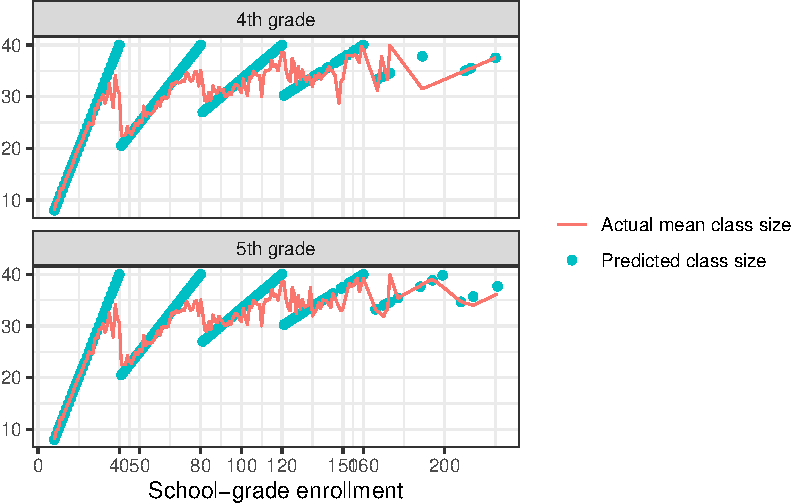
\includegraphics[keepaspectratio]{report_files/figure-pdf/unnamed-chunk-6-1.pdf}}

By overlaying actual and predicted average class size, we can see some
variations of actual class size from the predicted size. Still, we can
see there is some similar pattern happening in the actual case that is
analogous to the predicted class size. I did some calculations and found
that about 1\% of the sample are overshooters and about 3\% are early
splitters. It seems from the data that the early splitters usually have
bit more disadvantaged students and have studens with lower test scores
than the complying classes. The result is reverse for overshooters. Thus
for our RDD identification strategy to work, we would need to make sure
that these deviations are only marginal and there is not much cases
where schools can manipulate the number of class sizes in the cutoffs.

\subsection{Q5}\label{q5}

Results of the RDD estimates are as follows:

\begin{Shaded}
\begin{Highlighting}[]
\FunctionTok{library}\NormalTok{(glue)}
\FunctionTok{library}\NormalTok{(gt)}

\CommentTok{\# Define variables}
\NormalTok{test\_score\_vars }\OtherTok{\textless{}{-}} \FunctionTok{c}\NormalTok{(}\StringTok{"avgmath"}\NormalTok{, }\StringTok{"avgverb"}\NormalTok{)}
\NormalTok{bandwidths }\OtherTok{\textless{}{-}} \FunctionTok{c}\NormalTok{(}\DecValTok{2}\NormalTok{, }\DecValTok{5}\NormalTok{, }\DecValTok{8}\NormalTok{, }\DecValTok{10}\NormalTok{, }\DecValTok{15}\NormalTok{, }\DecValTok{20}\NormalTok{, }\DecValTok{25}\NormalTok{, }\DecValTok{30}\NormalTok{)}
\NormalTok{poly\_degs }\OtherTok{\textless{}{-}} \DecValTok{0}\SpecialCharTok{:}\DecValTok{4}

\ControlFlowTok{for}\NormalTok{ (test\_score }\ControlFlowTok{in}\NormalTok{ test\_score\_vars) \{}
  
  \CommentTok{\# Load dataset}
\NormalTok{  df }\OtherTok{\textless{}{-}}\NormalTok{ data }\SpecialCharTok{\%\textgreater{}\%}  
    \FunctionTok{mutate}\NormalTok{(}\AttributeTok{above\_cutoff\_1 =} \FunctionTok{as.integer}\NormalTok{(c\_size }\SpecialCharTok{\textgreater{}} \DecValTok{40}\NormalTok{))}
  
\NormalTok{  results }\OtherTok{\textless{}{-}} \FunctionTok{list}\NormalTok{()}
  
  \ControlFlowTok{for}\NormalTok{ (bw }\ControlFlowTok{in}\NormalTok{ bandwidths) \{}
\NormalTok{    df\_bw }\OtherTok{\textless{}{-}}\NormalTok{ df }\SpecialCharTok{\%\textgreater{}\%}
      \FunctionTok{filter}\NormalTok{(c\_size }\SpecialCharTok{\textgreater{}=}\NormalTok{ (}\DecValTok{40} \SpecialCharTok{{-}}\NormalTok{ bw), c\_size }\SpecialCharTok{\textless{}=}\NormalTok{ (}\DecValTok{40} \SpecialCharTok{+}\NormalTok{ bw))}

    \ControlFlowTok{for}\NormalTok{ (d }\ControlFlowTok{in}\NormalTok{ poly\_degs) \{}
      \CommentTok{\# Polynomial terms}
      \ControlFlowTok{if}\NormalTok{ (d }\SpecialCharTok{\textgreater{}} \DecValTok{0}\NormalTok{) \{}
        \ControlFlowTok{for}\NormalTok{ (i }\ControlFlowTok{in} \DecValTok{1}\SpecialCharTok{:}\NormalTok{d) \{}
\NormalTok{          poly\_var }\OtherTok{\textless{}{-}} \FunctionTok{paste0}\NormalTok{(}\StringTok{"c\_size\_"}\NormalTok{, i)}
          \ControlFlowTok{if}\NormalTok{ (}\SpecialCharTok{!}\NormalTok{(poly\_var }\SpecialCharTok{\%in\%} \FunctionTok{names}\NormalTok{(df\_bw))) \{}
\NormalTok{            df\_bw[[poly\_var]] }\OtherTok{\textless{}{-}}\NormalTok{ df\_bw}\SpecialCharTok{$}\NormalTok{c\_size}\SpecialCharTok{\^{}}\NormalTok{i}
\NormalTok{          \}}
\NormalTok{        \}}
\NormalTok{        covars }\OtherTok{\textless{}{-}} \FunctionTok{paste0}\NormalTok{(}\StringTok{"c\_size\_"}\NormalTok{, }\DecValTok{1}\SpecialCharTok{:}\NormalTok{d, }\AttributeTok{collapse =} \StringTok{"+"}\NormalTok{)}
\NormalTok{      \} }\ControlFlowTok{else}\NormalTok{ \{}
\NormalTok{        covars }\OtherTok{\textless{}{-}} \StringTok{"1"}
\NormalTok{      \}}
      
      \CommentTok{\# IV Regression using fixest}
\NormalTok{      formula\_iv }\OtherTok{\textless{}{-}} \FunctionTok{as.formula}\NormalTok{(}\FunctionTok{glue}\NormalTok{(}\StringTok{"\{test\_score\} \textasciitilde{} \{covars\} | classize \textasciitilde{} above\_cutoff\_1"}\NormalTok{))}
\NormalTok{      iv\_model }\OtherTok{\textless{}{-}} \FunctionTok{feols}\NormalTok{(formula\_iv, }\AttributeTok{data =}\NormalTok{ df\_bw, }\AttributeTok{cluster =} \SpecialCharTok{\textasciitilde{}}\NormalTok{schlcode)}
      
      \CommentTok{\# Store results}
\NormalTok{      results[[}\FunctionTok{length}\NormalTok{(results) }\SpecialCharTok{+} \DecValTok{1}\NormalTok{]] }\OtherTok{\textless{}{-}} \FunctionTok{tibble}\NormalTok{(}
        \AttributeTok{bandwidth =}\NormalTok{ bw,}
        \AttributeTok{degree =}\NormalTok{ d,}
        \AttributeTok{estimate =} \FunctionTok{coef}\NormalTok{(iv\_model)[}\StringTok{"fit\_classize"}\NormalTok{],}
        \AttributeTok{std\_error =} \FunctionTok{se}\NormalTok{(iv\_model)[}\StringTok{"fit\_classize"}\NormalTok{]}
\NormalTok{      )}
\NormalTok{    \}}
\NormalTok{  \}}
  
\NormalTok{  results\_df }\OtherTok{\textless{}{-}} \FunctionTok{bind\_rows}\NormalTok{(results)}


\CommentTok{\# Formatting output similar to Stata}
\NormalTok{  results\_formatted }\OtherTok{\textless{}{-}}\NormalTok{ results\_df }\SpecialCharTok{\%\textgreater{}\%}
    \FunctionTok{mutate}\NormalTok{(}
      \AttributeTok{estimate =} \FunctionTok{sprintf}\NormalTok{(}\StringTok{"\%.2f"}\NormalTok{, estimate),}
      \AttributeTok{std\_error =} \FunctionTok{sprintf}\NormalTok{(}\StringTok{"(\%.2f)"}\NormalTok{, std\_error)}
\NormalTok{    ) }\SpecialCharTok{\%\textgreater{}\%}
    \FunctionTok{pivot\_longer}\NormalTok{(}\AttributeTok{cols =} \FunctionTok{c}\NormalTok{(estimate, std\_error), }\AttributeTok{names\_to =} \StringTok{"type"}\NormalTok{, }\AttributeTok{values\_to =} \StringTok{"value"}\NormalTok{) }\SpecialCharTok{\%\textgreater{}\%}
    \FunctionTok{pivot\_wider}\NormalTok{(}\AttributeTok{names\_from =}\NormalTok{ bandwidth, }\AttributeTok{values\_from =}\NormalTok{ value, }\AttributeTok{names\_prefix =} \StringTok{"BW\_"}\NormalTok{) }\SpecialCharTok{\%\textgreater{}\%}
    \FunctionTok{arrange}\NormalTok{(degree, type) }\SpecialCharTok{\%\textgreater{}\%}
    \FunctionTok{mutate}\NormalTok{(}\AttributeTok{degree =} \FunctionTok{ifelse}\NormalTok{(type }\SpecialCharTok{==} \StringTok{"std\_error"}\NormalTok{, }\StringTok{""}\NormalTok{, }\FunctionTok{as.character}\NormalTok{(degree))) }\SpecialCharTok{\%\textgreater{}\%}
    \FunctionTok{select}\NormalTok{(}\SpecialCharTok{{-}}\NormalTok{type)}

  \CommentTok{\# Print formatted table using gt for Quarto}
\NormalTok{\}}
\end{Highlighting}
\end{Shaded}

\begin{table}
\fontsize{12.0pt}{14.4pt}\selectfont
\caption{RDD estimates of class size on math score}
\begin{tabular*}{\linewidth}{@{\extracolsep{\fill}}rrrrrrrrr}
\toprule
degree & BW\_2 & BW\_5 & BW\_8 & BW\_10 & BW\_15 & BW\_20 & BW\_25 & BW\_30 \\ 
\midrule\addlinespace[2.5pt]
0 & -0.21 & -0.33 & -0.29 & -0.32 & -0.58 & -1.77 & 1.72 & 0.82 \\ 
 & (0.27) & (0.19) & (0.18) & (0.17) & (0.24) & (0.91) & (0.81) & (0.25) \\ 
1 & -0.05 & -0.21 & -0.30 & -0.19 & -0.12 & -0.19 & -0.19 & -0.06 \\ 
 & (0.67) & (0.37) & (0.27) & (0.23) & (0.17) & (0.14) & (0.13) & (0.11) \\ 
2 & -0.13 & -0.23 & -0.39 & -0.31 & -0.16 & -0.21 & -0.24 & -0.20 \\ 
 & (0.68) & (0.37) & (0.29) & (0.24) & (0.17) & (0.14) & (0.12) & (0.11) \\ 
3 & 0.18 & 0.06 & -0.05 & -0.31 & -0.23 & -0.12 & -0.14 & -0.23 \\ 
 & (0.65) & (0.42) & (0.39) & (0.35) & (0.25) & (0.20) & (0.17) & (0.15) \\ 
4 & 0.18 & 0.06 & -0.07 & -0.31 & -0.40 & -0.17 & -0.14 & -0.21 \\ 
 & (0.57) & (0.42) & (0.39) & (0.35) & (0.28) & (0.21) & (0.18) & (0.16) \\ 
\bottomrule
\end{tabular*}
\end{table}

\begin{table}
\fontsize{12.0pt}{14.4pt}\selectfont
\caption{RDD estimates of class size on grammar score}
\begin{tabular*}{\linewidth}{@{\extracolsep{\fill}}rrrrrrrrr}
\toprule
degree & BW\_2 & BW\_5 & BW\_8 & BW\_10 & BW\_15 & BW\_20 & BW\_25 & BW\_30 \\ 
\midrule\addlinespace[2.5pt]
0 & -0.35 & -0.52 & -0.36 & -0.31 & -0.45 & -1.20 & 0.90 & 0.40 \\ 
 & (0.26) & (0.18) & (0.16) & (0.15) & (0.20) & (0.72) & (0.63) & (0.21) \\ 
1 & -0.70 & -0.39 & -0.57 & -0.47 & -0.30 & -0.29 & -0.25 & -0.14 \\ 
 & (0.67) & (0.35) & (0.25) & (0.22) & (0.15) & (0.13) & (0.11) & (0.10) \\ 
2 & -0.76 & -0.42 & -0.59 & -0.56 & -0.31 & -0.27 & -0.29 & -0.25 \\ 
 & (0.66) & (0.35) & (0.28) & (0.24) & (0.16) & (0.12) & (0.11) & (0.10) \\ 
3 & -0.52 & -0.25 & -0.45 & -0.63 & -0.50 & -0.38 & -0.35 & -0.35 \\ 
 & (0.79) & (0.38) & (0.39) & (0.34) & (0.25) & (0.19) & (0.16) & (0.14) \\ 
4 & -0.52 & -0.25 & -0.46 & -0.58 & -0.65 & -0.44 & -0.33 & -0.33 \\ 
 & (0.53) & (0.38) & (0.40) & (0.35) & (0.28) & (0.21) & (0.17) & (0.15) \\ 
\bottomrule
\end{tabular*}
\end{table}

\clearpage

Bandwidths (``BW'') restrict student enrollment to within a specified
number of students around the cutoff of 40. The estimates are sensitive
to the choice of bandwidth and polynomial degree, as the coefficients
vary considerably across specifications. Standard errors show that most
estimates are not statistically significantly different from zero,
although some become significant, especially when larger bandwidths are
used---likely due to the inclusion of more data points.

\subsection{Q6}\label{q6}

The replicated figure is as follows:

\begin{Shaded}
\begin{Highlighting}[]
\FunctionTok{library}\NormalTok{(rddensity)}
\FunctionTok{library}\NormalTok{(rdrobust)}

\CommentTok{\# Define grades to iterate over}
\NormalTok{grades }\OtherTok{\textless{}{-}} \DecValTok{4}\SpecialCharTok{:}\DecValTok{5}

\NormalTok{plots\_hist }\OtherTok{\textless{}{-}} \FunctionTok{list}\NormalTok{()}
\NormalTok{plots\_density }\OtherTok{\textless{}{-}} \FunctionTok{list}\NormalTok{()}

\ControlFlowTok{for}\NormalTok{ (g }\ControlFlowTok{in}\NormalTok{ grades) \{}
  \CommentTok{\# Load and process data}
\NormalTok{  df }\OtherTok{\textless{}{-}}\NormalTok{ data }\SpecialCharTok{\%\textgreater{}\%}
    \FunctionTok{filter}\NormalTok{(grade }\SpecialCharTok{==}\NormalTok{ g) }\SpecialCharTok{\%\textgreater{}\%}
    \FunctionTok{count}\NormalTok{(schlcode, c\_size, }\AttributeTok{name =} \StringTok{"freq"}\NormalTok{) }\SpecialCharTok{\%\textgreater{}\%}
    \FunctionTok{distinct}\NormalTok{(schlcode, }\AttributeTok{.keep\_all =} \ConstantTok{TRUE}\NormalTok{)}

  \CommentTok{\# Histogram plot}
\NormalTok{  hist\_plot }\OtherTok{\textless{}{-}} \FunctionTok{ggplot}\NormalTok{(df, }\FunctionTok{aes}\NormalTok{(}\AttributeTok{x =}\NormalTok{ c\_size)) }\SpecialCharTok{+}
    \FunctionTok{geom\_histogram}\NormalTok{(}\AttributeTok{binwidth =} \DecValTok{1}\NormalTok{, }\AttributeTok{fill =} \StringTok{"skyblue"}\NormalTok{, }\AttributeTok{color =} \StringTok{"black"}\NormalTok{) }\SpecialCharTok{+}
    \FunctionTok{geom\_vline}\NormalTok{(}\AttributeTok{xintercept =} \FunctionTok{c}\NormalTok{(}\DecValTok{40}\NormalTok{, }\DecValTok{80}\NormalTok{, }\DecValTok{120}\NormalTok{), }\AttributeTok{color =} \StringTok{"red"}\NormalTok{, }\AttributeTok{linetype =} \StringTok{"dashed"}\NormalTok{) }\SpecialCharTok{+}
    \FunctionTok{labs}\NormalTok{(}\AttributeTok{title =} \FunctionTok{paste0}\NormalTok{(g, }\StringTok{"th Grade Enrollment"}\NormalTok{), }\AttributeTok{x =} \StringTok{""}\NormalTok{, }\AttributeTok{y =} \StringTok{"Frequency"}\NormalTok{) }\SpecialCharTok{+}
    \FunctionTok{theme\_minimal}\NormalTok{()}

  \CommentTok{\# ggsave(filename = paste0("../output/hist\_", g, ".png"), plot = hist\_plot)}

\NormalTok{  plots\_hist[[}\FunctionTok{as.character}\NormalTok{(g)]] }\OtherTok{\textless{}{-}}\NormalTok{ hist\_plot}

  \CommentTok{\# McCrary density test plot}
\NormalTok{  mccrary }\OtherTok{\textless{}{-}} \FunctionTok{rddensity}\NormalTok{(df}\SpecialCharTok{$}\NormalTok{c\_size, }\AttributeTok{c =} \DecValTok{41}\NormalTok{)}
\NormalTok{  density\_plot }\OtherTok{\textless{}{-}} \FunctionTok{rdplotdensity}\NormalTok{(mccrary, df}\SpecialCharTok{$}\NormalTok{c\_size, }\AttributeTok{type =} \StringTok{"both"}\NormalTok{,}
                                \AttributeTok{title =} \FunctionTok{paste0}\NormalTok{(}\StringTok{"McCrary Density Test: Grade "}\NormalTok{, g))}

  \CommentTok{\# ggsave(filename = paste0("../output/mccrary\_", g, ".png"), plot = density\_plot$Estplot)}

\NormalTok{  plots\_density[[}\FunctionTok{as.character}\NormalTok{(g)]] }\OtherTok{\textless{}{-}}\NormalTok{ density\_plot}\SpecialCharTok{$}\NormalTok{Estplot}
\NormalTok{\}}
\end{Highlighting}
\end{Shaded}

\pandocbounded{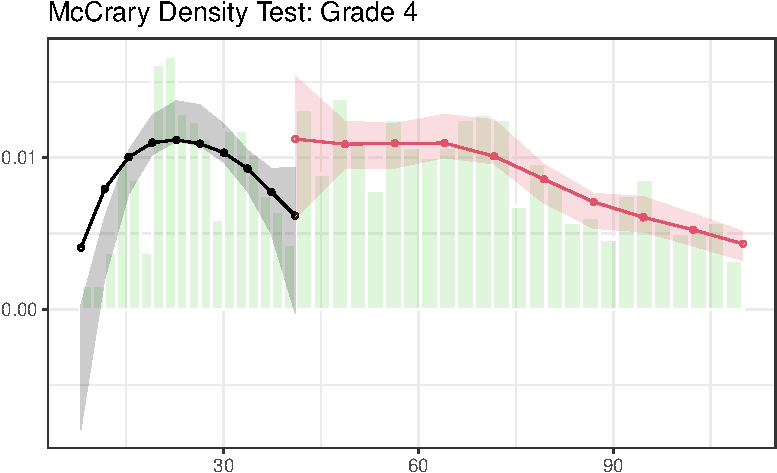
\includegraphics[keepaspectratio]{report_files/figure-pdf/unnamed-chunk-8-1.pdf}}

\pandocbounded{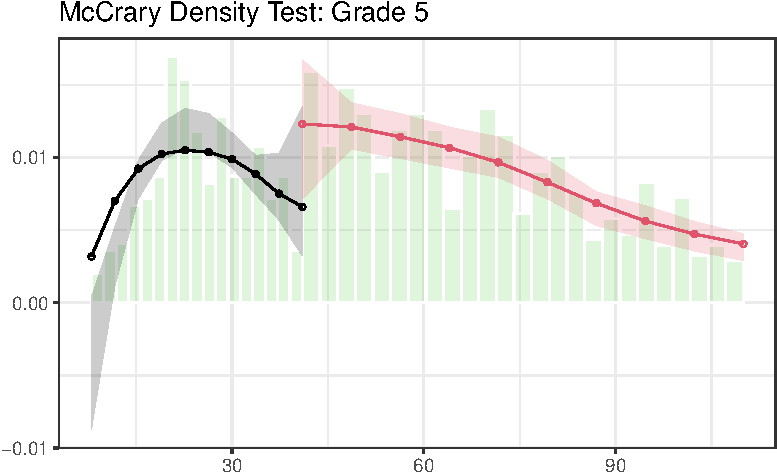
\includegraphics[keepaspectratio]{report_files/figure-pdf/unnamed-chunk-8-2.pdf}}

\begin{Shaded}
\begin{Highlighting}[]
\CommentTok{\# Combine plots using patchwork}
\FunctionTok{library}\NormalTok{(patchwork)}

\NormalTok{final\_plot }\OtherTok{\textless{}{-}}\NormalTok{ (plots\_hist[[}\StringTok{"5"}\NormalTok{]] }\SpecialCharTok{+}\NormalTok{ plots\_hist[[}\StringTok{"4"}\NormalTok{]]) }\SpecialCharTok{/}\NormalTok{ (plots\_density[[}\StringTok{"5"}\NormalTok{]] }\SpecialCharTok{+}\NormalTok{ plots\_density[[}\StringTok{"4"}\NormalTok{]])}

\NormalTok{final\_plot}
\end{Highlighting}
\end{Shaded}

\pandocbounded{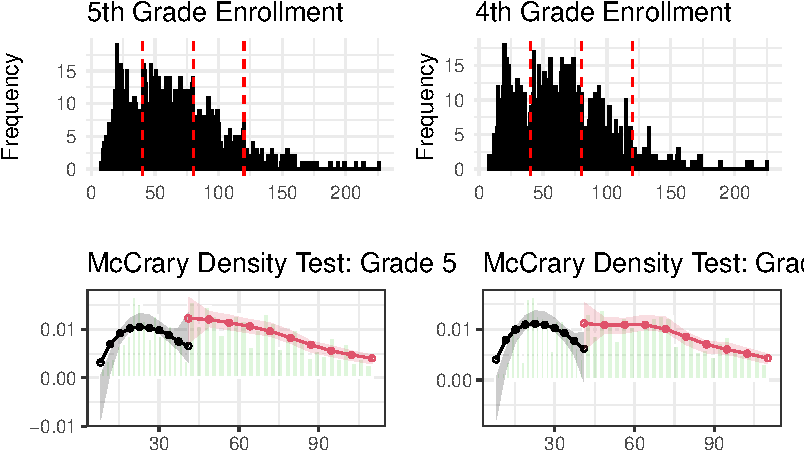
\includegraphics[keepaspectratio]{report_files/figure-pdf/unnamed-chunk-8-3.pdf}}

We should interpret these jumps as the sign of manipulation of the
running variable at the threshold, which can invalidate the identifying
assumption of the RDD.\footnote{Note that the graph looks bit different
  than the paper because I am using R package.}

\subsection{Q7}\label{q7}

I have replicated the table as follows:

\begin{Shaded}
\begin{Highlighting}[]
\FunctionTok{library}\NormalTok{(glue)}

\CommentTok{\# Load and prepare data}
\NormalTok{df }\OtherTok{\textless{}{-}}\NormalTok{ data }\SpecialCharTok{\%\textgreater{}\%}  
  \FunctionTok{mutate}\NormalTok{(}
    \AttributeTok{pred\_num\_classes =} \FunctionTok{floor}\NormalTok{((c\_size }\SpecialCharTok{{-}} \DecValTok{1}\NormalTok{) }\SpecialCharTok{/} \DecValTok{40}\NormalTok{) }\SpecialCharTok{+} \DecValTok{1}\NormalTok{,}
    \AttributeTok{pred\_class\_size =}\NormalTok{ c\_size }\SpecialCharTok{/}\NormalTok{ pred\_num\_classes,}
    \AttributeTok{above\_cutoff\_1 =} \FunctionTok{as.integer}\NormalTok{(c\_size }\SpecialCharTok{\textgreater{}} \DecValTok{40}\NormalTok{),}
    \AttributeTok{c\_size\_2\_d100 =}\NormalTok{ (c\_size}\SpecialCharTok{\^{}}\DecValTok{2}\NormalTok{) }\SpecialCharTok{/} \DecValTok{100}
\NormalTok{  )}

\NormalTok{grades }\OtherTok{\textless{}{-}} \FunctionTok{c}\NormalTok{(}\DecValTok{5}\NormalTok{, }\DecValTok{4}\NormalTok{)}
\NormalTok{donut\_widths }\OtherTok{\textless{}{-}} \FunctionTok{c}\NormalTok{(}\DecValTok{1}\NormalTok{, }\DecValTok{2}\NormalTok{, }\DecValTok{3}\NormalTok{)}

\NormalTok{results }\OtherTok{\textless{}{-}} \FunctionTok{list}\NormalTok{()}

\ControlFlowTok{for}\NormalTok{ (g }\ControlFlowTok{in}\NormalTok{ grades) \{}
  \ControlFlowTok{for}\NormalTok{ (dw }\ControlFlowTok{in}\NormalTok{ donut\_widths) \{}
\NormalTok{    df\_donut }\OtherTok{\textless{}{-}}\NormalTok{ df }\SpecialCharTok{\%\textgreater{}\%}
      \FunctionTok{filter}\NormalTok{((c\_size }\SpecialCharTok{\textless{}} \DecValTok{40} \SpecialCharTok{{-}}\NormalTok{ dw }\SpecialCharTok{|}\NormalTok{ c\_size }\SpecialCharTok{\textgreater{}} \DecValTok{40} \SpecialCharTok{+}\NormalTok{ dw) }\SpecialCharTok{\&}\NormalTok{ grade }\SpecialCharTok{==}\NormalTok{ g)}

    \CommentTok{\# Language {-} no quad term}
\NormalTok{    mod1 }\OtherTok{\textless{}{-}} \FunctionTok{feols}\NormalTok{(avgverb }\SpecialCharTok{\textasciitilde{}}\NormalTok{ tipuach }\SpecialCharTok{+}\NormalTok{ c\_size }\SpecialCharTok{|}\NormalTok{ classize }\SpecialCharTok{\textasciitilde{}}\NormalTok{ pred\_class\_size, }\AttributeTok{data =}\NormalTok{ df\_donut, }\AttributeTok{cluster =} \SpecialCharTok{\textasciitilde{}}\NormalTok{schlcode)}
\NormalTok{    l1\_b }\OtherTok{\textless{}{-}} \FunctionTok{coef}\NormalTok{(mod1)[}\StringTok{"fit\_classize"}\NormalTok{]}
\NormalTok{    l1\_se }\OtherTok{\textless{}{-}} \FunctionTok{se}\NormalTok{(mod1)[}\StringTok{"fit\_classize"}\NormalTok{]}

    \CommentTok{\# Language {-} with quad term}
\NormalTok{    mod2 }\OtherTok{\textless{}{-}} \FunctionTok{feols}\NormalTok{(avgverb }\SpecialCharTok{\textasciitilde{}}\NormalTok{ tipuach }\SpecialCharTok{+}\NormalTok{ c\_size }\SpecialCharTok{+}\NormalTok{ c\_size\_2\_d100 }\SpecialCharTok{|}\NormalTok{ classize }\SpecialCharTok{\textasciitilde{}}\NormalTok{ pred\_class\_size, }\AttributeTok{data =}\NormalTok{ df\_donut, }\AttributeTok{cluster =} \SpecialCharTok{\textasciitilde{}}\NormalTok{schlcode)}
\NormalTok{    l2\_b }\OtherTok{\textless{}{-}} \FunctionTok{coef}\NormalTok{(mod2)[}\StringTok{"fit\_classize"}\NormalTok{]}
\NormalTok{    l2\_se }\OtherTok{\textless{}{-}} \FunctionTok{se}\NormalTok{(mod2)[}\StringTok{"fit\_classize"}\NormalTok{]}

    \CommentTok{\# Math {-} no quad term}
\NormalTok{    mod3 }\OtherTok{\textless{}{-}} \FunctionTok{feols}\NormalTok{(avgmath }\SpecialCharTok{\textasciitilde{}}\NormalTok{ tipuach }\SpecialCharTok{+}\NormalTok{ c\_size }\SpecialCharTok{|}\NormalTok{ classize }\SpecialCharTok{\textasciitilde{}}\NormalTok{ pred\_class\_size, }\AttributeTok{data =}\NormalTok{ df\_donut, }\AttributeTok{cluster =} \SpecialCharTok{\textasciitilde{}}\NormalTok{schlcode)}
\NormalTok{    m3\_b }\OtherTok{\textless{}{-}} \FunctionTok{coef}\NormalTok{(mod3)[}\StringTok{"fit\_classize"}\NormalTok{]}
\NormalTok{    m3\_se }\OtherTok{\textless{}{-}} \FunctionTok{se}\NormalTok{(mod3)[}\StringTok{"fit\_classize"}\NormalTok{]}

    \CommentTok{\# Math {-} with quad term}
\NormalTok{    mod4 }\OtherTok{\textless{}{-}} \FunctionTok{feols}\NormalTok{(avgmath }\SpecialCharTok{\textasciitilde{}}\NormalTok{ tipuach }\SpecialCharTok{+}\NormalTok{ c\_size }\SpecialCharTok{+}\NormalTok{ c\_size\_2\_d100 }\SpecialCharTok{|}\NormalTok{ classize }\SpecialCharTok{\textasciitilde{}}\NormalTok{ pred\_class\_size, }\AttributeTok{data =}\NormalTok{ df\_donut, }\AttributeTok{cluster =} \SpecialCharTok{\textasciitilde{}}\NormalTok{schlcode)}
\NormalTok{    m4\_b }\OtherTok{\textless{}{-}} \FunctionTok{coef}\NormalTok{(mod4)[}\StringTok{"fit\_classize"}\NormalTok{]}
\NormalTok{    m4\_se }\OtherTok{\textless{}{-}} \FunctionTok{se}\NormalTok{(mod4)[}\StringTok{"fit\_classize"}\NormalTok{]}

\NormalTok{    results[[}\FunctionTok{length}\NormalTok{(results)}\SpecialCharTok{+}\DecValTok{1}\NormalTok{]] }\OtherTok{\textless{}{-}} \FunctionTok{tibble}\NormalTok{(}
      \AttributeTok{grade =} \FunctionTok{as.character}\NormalTok{(g), }\AttributeTok{donut =} \FunctionTok{as.character}\NormalTok{(dw), }\AttributeTok{est\_type =} \StringTok{"Estimate"}\NormalTok{,}
      \AttributeTok{lang1 =} \FunctionTok{sprintf}\NormalTok{(}\StringTok{"\%.4f"}\NormalTok{, l1\_b),}
      \AttributeTok{lang2 =} \FunctionTok{sprintf}\NormalTok{(}\StringTok{"\%.4f"}\NormalTok{, l2\_b),}
      \AttributeTok{math1 =} \FunctionTok{sprintf}\NormalTok{(}\StringTok{"\%.4f"}\NormalTok{, m3\_b),}
      \AttributeTok{math2 =} \FunctionTok{sprintf}\NormalTok{(}\StringTok{"\%.4f"}\NormalTok{, m4\_b)}
\NormalTok{    )}

\NormalTok{    results[[}\FunctionTok{length}\NormalTok{(results)}\SpecialCharTok{+}\DecValTok{1}\NormalTok{]] }\OtherTok{\textless{}{-}} \FunctionTok{tibble}\NormalTok{(}
      \AttributeTok{grade =} \StringTok{""}\NormalTok{, }\AttributeTok{donut =} \StringTok{""}\NormalTok{, }\AttributeTok{est\_type =} \StringTok{"SE"}\NormalTok{,}
      \AttributeTok{lang1 =} \FunctionTok{glue}\NormalTok{(}\StringTok{"(\{sprintf(\textquotesingle{}\%.4f\textquotesingle{}, l1\_se)\})"}\NormalTok{),}
      \AttributeTok{lang2 =} \FunctionTok{glue}\NormalTok{(}\StringTok{"(\{sprintf(\textquotesingle{}\%.4f\textquotesingle{}, l2\_se)\})"}\NormalTok{),}
      \AttributeTok{math1 =} \FunctionTok{glue}\NormalTok{(}\StringTok{"(\{sprintf(\textquotesingle{}\%.4f\textquotesingle{}, m3\_se)\})"}\NormalTok{),}
      \AttributeTok{math2 =} \FunctionTok{glue}\NormalTok{(}\StringTok{"(\{sprintf(\textquotesingle{}\%.4f\textquotesingle{}, m4\_se)\})"}\NormalTok{)}
\NormalTok{    )}
\NormalTok{  \}}
\NormalTok{\}}

\NormalTok{result\_df }\OtherTok{\textless{}{-}} \FunctionTok{bind\_rows}\NormalTok{(results) }\SpecialCharTok{\%\textgreater{}\%}
  \FunctionTok{mutate}\NormalTok{(}
    \AttributeTok{donut\_int =} \FunctionTok{ifelse}\NormalTok{(est\_type }\SpecialCharTok{==} \StringTok{"Estimate"}\NormalTok{, }\FunctionTok{paste0}\NormalTok{(}\StringTok{"["}\NormalTok{, }\DecValTok{40} \SpecialCharTok{{-}} \FunctionTok{as.numeric}\NormalTok{(donut), }\StringTok{","}\NormalTok{, }\DecValTok{40} \SpecialCharTok{+} \FunctionTok{as.numeric}\NormalTok{(donut), }\StringTok{"]"}\NormalTok{), }\StringTok{""}\NormalTok{),}
    \AttributeTok{grade =} \FunctionTok{ifelse}\NormalTok{(est\_type }\SpecialCharTok{==} \StringTok{"SE"}\NormalTok{, }\StringTok{""}\NormalTok{, grade)}
\NormalTok{  ) }\SpecialCharTok{\%\textgreater{}\%}
  \FunctionTok{select}\NormalTok{(grade, donut\_int, lang1, lang2, math1, math2)}

\CommentTok{\# Add manual footnotes}
\NormalTok{manual\_notes }\OtherTok{\textless{}{-}} \FunctionTok{tibble}\NormalTok{(}
  \AttributeTok{grade =} \FunctionTok{c}\NormalTok{(}\StringTok{"Controls:"}\NormalTok{, }\StringTok{"Percent Disadvantaged"}\NormalTok{, }\StringTok{"Enrollment"}\NormalTok{, }\StringTok{"Enrollment Squared /100"}\NormalTok{),}
  \AttributeTok{donut\_int =} \FunctionTok{c}\NormalTok{(}\StringTok{""}\NormalTok{, }\StringTok{""}\NormalTok{, }\StringTok{""}\NormalTok{, }\StringTok{""}\NormalTok{),}
  \AttributeTok{lang1 =} \FunctionTok{c}\NormalTok{(}\StringTok{""}\NormalTok{, }\StringTok{"X"}\NormalTok{, }\StringTok{"X"}\NormalTok{, }\StringTok{""}\NormalTok{),}
  \AttributeTok{lang2 =} \FunctionTok{c}\NormalTok{(}\StringTok{""}\NormalTok{, }\StringTok{"X"}\NormalTok{, }\StringTok{"X"}\NormalTok{, }\StringTok{"X"}\NormalTok{),}
  \AttributeTok{math1 =} \FunctionTok{c}\NormalTok{(}\StringTok{""}\NormalTok{, }\StringTok{"X"}\NormalTok{, }\StringTok{"X"}\NormalTok{, }\StringTok{""}\NormalTok{),}
  \AttributeTok{math2 =} \FunctionTok{c}\NormalTok{(}\StringTok{""}\NormalTok{, }\StringTok{"X"}\NormalTok{, }\StringTok{"X"}\NormalTok{, }\StringTok{"X"}\NormalTok{)}
\NormalTok{)}

\NormalTok{final\_table }\OtherTok{\textless{}{-}} \FunctionTok{bind\_rows}\NormalTok{(result\_df, manual\_notes)}

\CommentTok{\# Display table in Quarto{-}friendly format}
\NormalTok{knitr}\SpecialCharTok{::}\FunctionTok{kable}\NormalTok{(}
\NormalTok{  final\_table,}
  \AttributeTok{format =} \StringTok{"latex"}\NormalTok{,}
  \AttributeTok{booktabs =} \ConstantTok{TRUE}\NormalTok{,}
  \AttributeTok{caption =} \StringTok{"Replication of Table A6"}
\NormalTok{)}
\end{Highlighting}
\end{Shaded}

\begin{table}

\caption{Replication of Table A6}
\centering
\begin{tabular}[t]{llllll}
\toprule
grade & donut\_int & lang1 & lang2 & math1 & math2\\
\midrule
5 & {}[39,41] & -0.2341 & -0.2010 & -0.1704 & -0.1977\\
 &  & (0.0763) & (0.0956) & (0.1041) & (0.1313)\\
5 & {}[38,42] & -0.2406 & -0.2072 & -0.1743 & -0.2034\\
 &  & (0.0777) & (0.0988) & (0.1069) & (0.1376)\\
5 & {}[37,43] & -0.2152 & -0.1696 & -0.1659 & -0.1833\\
\addlinespace
 &  & (0.0778) & (0.0992) & (0.1082) & (0.1398)\\
4 & {}[39,41] & -0.1267 & -0.0581 & -0.0544 & -0.0353\\
 &  & (0.0613) & (0.0691) & (0.0749) & (0.0860)\\
4 & {}[38,42] & -0.1187 & -0.0431 & -0.0438 & -0.0208\\
 &  & (0.0632) & (0.0720) & (0.0776) & (0.0901)\\
\addlinespace
4 & {}[37,43] & -0.1166 & -0.0390 & -0.0467 & -0.0227\\
 &  & (0.0650) & (0.0744) & (0.0795) & (0.0928)\\
Controls: &  &  &  &  & \\
Percent Disadvantaged &  & X & X & X & X\\
Enrollment &  & X & X & X & X\\
\addlinespace
Enrollment Squared /100 &  &  & X &  & X\\
\bottomrule
\end{tabular}
\end{table}

This result shows us that the estimates are pretty close to the
estimates that Angrist et al.~(2019) replicated in their Table A4. This
result is not senstiive to the change in the width of the donut or the
type of test score. This implies that the manipulation of enrollment
counts near the threshold does not significantly affect the estimates of
interest. This suggests that we do not need to worry too much about the
bunching problem around the cutoff.




\end{document}
